% 03a_device_circuit_models.tex
% Manuscript RENDER of KB leaf ave-kb/vol9/ch3-pin-port-configuration/device-circuit-models.md
% Source of truth: the KB leaf. This file supplies PDF figures + \kbleaf{} wiring only.

\section{Device Circuit Models}
\label{sec:vol9_device_circuit_models}

\noindent\textbf{Canonical source (KB).} All spec tables, port assignments, and discipline notes for this section live in \kbleaf{ave-kb/vol9/ch3-pin-port-configuration/device-circuit-models.md}. The subsections below reproduce the figure set for the PDF; edit the KB leaf first, then sync any numeric table rows here if the render must stay byte-identical.

\subsection{Universal Vacuum Cell (\texttt{AVE\_VACUUM\_CELL})}
\label{sec:vol9_ave_vacuum_cell_circuit}

% circuit_vacuum_cell.tex — AVE_VACUUM_CELL schematic (Vol 9 Ch.3)
% Included from chapters/03_pin_port_configuration.tex
\begin{figure}[htbp]
\centering
\begin{circuitikz}[american, scale=0.95, transform shape]
    % Terminals
    \draw (0,0) node[left] {A} to[short, o-] (1,0);
    \draw (7,0) node[right] {B} to[short, o-] (8,0);

    % Relativistic inductor branch (series L + behavioral correction)
    \draw (1,0) to[L, l=$L_0$, i=$I$] (3.5,0);

    % Metric varactor (shunt nonlinear C)
    \draw (3.5,0) to[short] (5.5,0);
    \draw (4.5,0) to[C, l=$C_{\mathrm{eff}}(V)$, *-] (4.5,-1.8) node[ground] {};

    % Optional damping (dashed)
    \draw[dashed, gray] (1,0) to[R, l=\scriptsize $R_0$] (1,-1.2) node[ground] {};
    \draw (5.5,0) to[short] (7,0);

    % Annotations
    \node[align=center, font=\scriptsize] at (4.5, 1.35) {Metric varactor: $C_{\mathrm{eff}} = C_0/S(V)$};
    \node[align=center, font=\scriptsize] at (2.25, 1.0) {Relativistic inductor: $L_{\mathrm{eff}}(I)$};
    \node[align=center, font=\scriptsize] at (4.5, -2.55) {TVS / rupture at $|V| \ge V_{\mathrm{yield}}$ (optional)};
\end{circuitikz}
\caption{\texttt{AVE\_VACUUM\_CELL} schematic (Vol.~9 Ch.~3 device-circuit-models \S1; SPICE subcircuit Vol.~4 Ch.~18). Canonical leaves cited in \S\ref{sec:vol9_device_circuit_models}.}
\label{fig:vol9_circuit_vacuum_cell}
\end{figure}


\subsection{Electron Device: TIR-Confined LC Tank}
\label{sec:vol9_electron_device_circuit}

% circuit_electron_barrier.tex — Electron TIR-confined LC tank (Vol 9 Ch.3)
\begin{figure}[htbp]
\centering
\begin{circuitikz}[american, scale=0.9, transform shape]
    % Cold vacuum transmission lines (Z_EM = Z_0)
    \draw (0,0) node[left, align=right, font=\scriptsize] {vacuum\\$Z_{\mathrm{EM}}=Z_0$}
        to[short, o-] (1.2,0);
    \draw (10.8,0) to[short, o-] (12,0)
        node[right, align=left, font=\scriptsize] {vacuum\\$Z_{\mathrm{EM}}=Z_0$};

    % Left saturation barrier (bulk-channel TIR)
    \draw[thick, red!70!black] (1.2,0) -- (1.2,0.9) -- (2.0,0.9) -- (2.0,-0.9) -- (1.2,-0.9) -- (1.2,0);
    \node[font=\scriptsize, red!70!black, align=center] at (1.6, 1.55) {$\Gamma_{\mathrm{bulk}}=-1$\\$Z_{\mathrm{bulk}}\!\to\!0$};

    % Right barrier
    \draw[thick, red!70!black] (10.0,0) -- (10.0,0.9) -- (10.8,0.9) -- (10.8,-0.9) -- (10.0,-0.9) -- (10.0,0);
    \node[font=\scriptsize, red!70!black, align=center] at (10.4, 1.55) {$\Gamma_{\mathrm{bulk}}=-1$\\$Z_{\mathrm{bulk}}\!\to\!0$};

    % Confined LC tank (bond pair at ell_node)
    \draw (2.0,0) to[short] (4.0,0);
    \draw (4.0,0) to[L, l=$L_{\mathrm{cell}}$, i=$i$] (6.0,0);
    \draw (6.0,0) to[short] (8.0,0);
    \draw (7.0,0) to[C, l=$C_{\mathrm{eff}}$, *-] (7.0,-1.6) node[ground] {};
    \draw (8.0,0) to[short] (10.0,0);

    % Tank labels
    \node[align=center, font=\scriptsize] at (6.0, 1.35) {Electron LC tank at $\ell_{\mathrm{node}}$};
    \node[align=center, font=\scriptsize] at (6.0, -2.35) {$\omega_C = c_0/\ell_{\mathrm{node}}$ \quad $Q_{\mathrm{tank}} \approx \alpha^{-1}$};
    \node[align=center, font=\scriptsize, blue!60!black] at (6.0, -3.05) {Phase-space $(2,3)$ winding on Clifford torus; real-space $0_1$ unknot body};

    % Reactive store callout
    \draw[dashed, gray] (7.0,-1.6) -- (7.0,-3.8);
    \node[align=center, font=\scriptsize, gray] at (9.2, -3.8) {$Q_{\mathrm{react}} = m_e c^2 \cdot \alpha$};
\end{circuitikz}
\caption{Electron $\Gamma_{\mathrm{bulk}}=-1$ LC tank (Vol.~9 Ch.~3 \S2). Astrophysical bulk impedance at saturation boundary: Vol.~3 Ch.~15 KB leaf (see \S\ref{sec:vol9_device_circuit_models}).}
\label{fig:vol9_circuit_electron_barrier}
\end{figure}


\subsubsection{Operating-point coefficients at $A^2 \approx 0.23$}
\label{subsec:vol9_electron_op_coefficients}

Values from \kbleaf{ave-kb/vol9/ch3-pin-port-configuration/device-circuit-models.md} (driver \texttt{operating\_point\_coefficients.py}; consistency-class):

\begin{table}[htbp]
\centering\footnotesize
\begin{tabular}{@{}l l l@{}}
\toprule
\textbf{Quantity} & \textbf{Value} & \textbf{Regime / note} \\
\midrule
$A^2$ & $0.23$ & Regime II (nonlinear tensor) \\
$S(A)$ & $0.877$ & Sub-yield, pre-rupture \\
$C_{\mathrm{eff}}/C_0$ & $1.140$ & Metric varactor slope active \\
$\mathrm{d}(C_{\mathrm{eff}}/C_0)/\mathrm{d}A$ & $0.710$ & Datasheet nonlinearity column \\
$Q$ (at $\gamma = \alpha\,\omega_C$) & $\approx 137$ & Loss carries $\alpha$ (consistency) \\
$V_{\mathrm{op}}$ & $\approx 20.9$~kV & $48\%$ of $V_{\mathrm{yield}}$ \\
\bottomrule
\end{tabular}
\caption{Electron-device operating-point coefficients (KB-sourced). Emergence gate for $Q = 1/\alpha$: real dark-wake $\tau_{zx}$, not toy loss.}
\label{tab:vol9_electron_op_coefficients}
\end{table}

\subsection{Three-Channel Boundary Port}
\label{sec:vol9_three_channel_circuit}

% circuit_three_channel_boundary.tex — Three-impedance port at one boundary (Vol 9 Ch.3)
\begin{figure}[htbp]
\centering
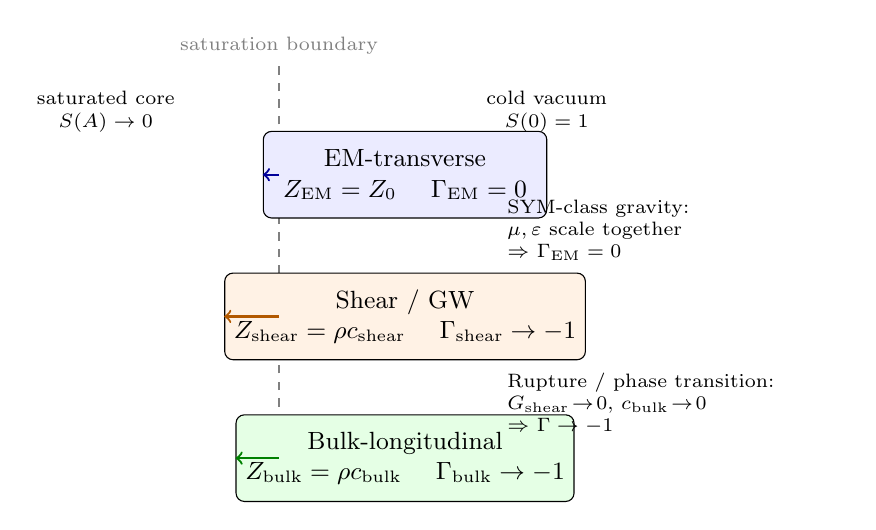
\begin{tikzpicture}[
    port/.style={draw, rounded corners=3pt, minimum width=3.6cm, minimum height=1.1cm, align=center, font=\small},
    line/.style={thick},
    arr/.style={->, thick}
]
    % Boundary plane
    \draw[line, dashed, gray] (0,-2.2) -- (0,3.2) node[above, font=\scriptsize, gray] {saturation boundary};

    % Interior (saturated core)
    \node[font=\scriptsize, align=center] at (-2.2, 2.6) {saturated core\\$S(A)\to 0$};

    % Exterior (cold vacuum)
    \node[font=\scriptsize, align=center] at (3.4, 2.6) {cold vacuum\\$S(0)=1$};

    % Three channel ports
    \node[port, fill=blue!8] (em) at (1.6, 1.8) {EM-transverse\\$Z_{\mathrm{EM}} = Z_0$ \quad $\Gamma_{\mathrm{EM}} = 0$};
    \node[port, fill=orange!10] (sh) at (1.6, 0) {Shear / GW\\$Z_{\mathrm{shear}} = \rho c_{\mathrm{shear}}$ \quad $\Gamma_{\mathrm{shear}} \to -1$};
    \node[port, fill=green!10] (bk) at (1.6, -1.8) {Bulk-longitudinal\\$Z_{\mathrm{bulk}} = \rho c_{\mathrm{bulk}}$ \quad $\Gamma_{\mathrm{bulk}} \to -1$};

    % Arrows from boundary
    \draw[arr, blue!60!black] (0,1.8) -- (em.west);
    \draw[arr, orange!70!black] (0,0) -- (sh.west);
    \draw[arr, green!50!black] (0,-1.8) -- (bk.west);

    % SYM note for EM at gravity boundary
    \node[font=\scriptsize, align=left, text width=4.2cm] at (5.0, 1.1) {SYM-class gravity:\\$\mu,\varepsilon$ scale together\\$\Rightarrow$ $\Gamma_{\mathrm{EM}}=0$};

    % Rupture note for shear/bulk
    \node[font=\scriptsize, align=left, text width=4.2cm] at (5.0, -1.1) {Rupture / phase transition:\\$G_{\mathrm{shear}}\!\to\!0$, $c_{\mathrm{bulk}}\!\to\!0$\\$\Rightarrow$ $\Gamma \to -1$};
\end{tikzpicture}
\caption{Three-channel boundary port (Vol.~9 Ch.~3 \S3; DC impedances Ch.~4). Canonical tables in \S\ref{sec:vol9_device_circuit_models}.}
\label{fig:vol9_circuit_three_channel}
\end{figure}


\subsection{Cascaded Vacuum Line (Device String)}
\label{sec:vol9_cascaded_vacuum_line}

\begin{figure}[htbp]
\centering
\begin{circuitikz}[american, scale=0.85, transform shape]
    \draw (0,0) node[left] {IN} to[short, o-] (0.8,0);
    \node[draw, minimum width=1.6cm, minimum height=0.9cm, font=\scriptsize] (x1) at (2.0,0) {cell};
    \draw (0.8,0) -- (x1.west);
    \node[draw, minimum width=1.6cm, minimum height=0.9cm, font=\scriptsize] (x2) at (4.5,0) {cell};
    \draw (x1.east) -- (x2.west);
    \node[draw, minimum width=1.6cm, minimum height=0.9cm, font=\scriptsize] (x3) at (7.0,0) {cell};
    \draw (x2.east) -- (x3.west);
    \draw (x3.east) to[short, o-] (8.2,0) node[right] {OUT};
    \node[font=\scriptsize] at (4.5, -1.1) {$N$ cascaded \texttt{AVE\_VACUUM\_CELL} bonds $\Rightarrow$ distributed K4-TLM line};
    \draw[dashed, gray] (0.8,-1.8) -- (8.2,-1.8);
    \node[font=\scriptsize, gray] at (4.5, -2.35) {Each cell: $L_0=\mu_0\ell_{\mathrm{node}}$, $C_0=\varepsilon_0\ell_{\mathrm{node}}$, $Z_0=\sqrt{L_0/C_0}$};
\end{circuitikz}
\caption{Cascaded vacuum-cell device string (Vol.~9 Ch.~3 device-circuit-models \S4).}
\label{fig:vol9_cascaded_vacuum_line}
\end{figure}
